\documentclass[AMS,STIX2COL]{WileyNJD-v2}

\articletype{Article Type}%

\received{26 April 2016}
\revised{6 June 2016}
\accepted{6 June 2016}

\raggedbottom


\begin{document}

    \title{Improvement of Korean Morphological Analysis System Through Transformer-based Re-ranking}

    \author[1]{Author One*}

    \author[2,3]{Author Two}

    \author[3]{Author Three}

    \authormark{AUTHOR ONE \textsc{et al}}


    \address[1]{\orgdiv{Org Division}, \orgname{Org Name}, \orgaddress{\state{State name}, \country{Country name}}}

    \address[2]{\orgdiv{Org Division}, \orgname{Org Name}, \orgaddress{\state{State name}, \country{Country name}}}

    \address[3]{\orgdiv{Org Division}, \orgname{Org Name}, \orgaddress{\state{State name}, \country{Country name}}}

    \corres{*Corresponding author name, This is sample corresponding address. \email{authorone@gmail.com}}

    \presentaddress{This is sample for present address text this is sample for present address text}

    \abstract[Abstract]{
        Korean morphological analysis plays a basic and important role enough to be called the first step in Korean language analysis.
        Due to the nature of Korean agglutinative words, it was difficult to build an automatic analysis system because the analysis was not completed with part-of-speech tagging alone, as in English.
        In addition, various methods for morphological analysis have been proposed, but efficient methods such as BPE are mainly used in applications intended to be used as tokenizers for deep learning.
        In this paper, we propose a method to maximize the performance of an efficient morphological analysis system that can be used for tokenization through multi-stage re-ranking based on deep learning.
        For a number of various cases whose rankings have been changed through re-ranking, it is possible to improve performance while maintaining speed by updating the cost matrix of the lattice-based morphological analysis system in the future.
        Through experiments, we showed that the proposed method effectively improved performance by reducing errors by more than 40\% in both the spoken language model and the written language model.
    }
    %한국어 형태소 분석은 한국어 분석의 첫걸음이라고 할 정도로 기본적이고 중요한 역할을 담당하고 있다.
    %한국어는 교착어의 특성으로 인해 영어처럼 품사 태깅만으로는 분석이 끝나지 않아 자동 분석 시스템 구축에 어려움이 있어왔다.
    %또한 형태소분석을 위한 다양한 방법들이 제안되었지만, 딥러닝을 위한 토큰화기로 활용하려는 응용에서는 BPE와 같은 효율적인 방법들이 주로 사용되고 있다.
    %본 논문에서는 토큰화에서도 사용이 가능한 효율적인 형태소분석 시스템의 성능을 딥러닝 기반의 Multi-Stage 재순위화를 통해 극대화하는 방법에 대해 제안하고자 한다.
    %재순위화를 통해 순위가 바뀌어진 다수의 다양한 사례들은 추후 Lattice 기반 형태소분석 시스템의 cost matrix를 업데이트함으로 속도를 유지하면서 성능을 개선하는 것이 가능해진다.
    %실험을 통해 제안하는 방법을 통해 구어체 모델과 문어체 모델에서 모두 기존보다 오류가 40% 이상 감소됨 보임으로 제안한 방법이 효과적으로 성능을 개선하였음을 보였다.

    \keywords{keyword1, keyword2, keyword3, keyword4}

    \JELinfo{classification}

    \MSC{Code numbers}

    \jnlcitation{\cname{%
        \author{Williams K.},
        \author{B. Hoskins},
        \author{R. Lee},
        \author{G. Masato}, and \author{T. Woollings}} (\cyear{2016}),
        \ctitle{A regime analysis of Atlantic winter jet variability applied to evaluate HadGEM3-GC2}, \cjournal{Q.J.R. Meteorol. Soc.}, \cvol{2017;00:1--6}.}


    \maketitle

    \footnotetext{\textbf{Abbreviations:} ANA, anti-nuclear antibodies; APC, antigen-presenting cells; IRF, interferon regulatory factor}


    \section{Introduction}\label{sec1}

    Korean morphological analysis is the process of determining parts of speech by finding morphemes, which are the smallest units of language expression that have an independent meaning in a sentence.
    In an isolating language like English, this can be done relatively simply by tagging parts of speech sequentially, but in Korean, the nature of the agglutinative language requires separating endings or investigatives and restoring inflections to their original form.
    In addition, since the basic input of other Korean analysis tasks is often a separated morpheme, the accuracy of morphological analysis greatly affects the performance of Korean analysis.
    Modern, high-performance deep learning methods in natural language processing use a tokenisation process that breaks text into smaller units, and then converts each token into a vector as input to the computational model~\cite{Mikolov2013}.
    In this case, the token unit is mainly subword units, and to reflect the characteristics of Korean, subword tokenisation is attempted with separated morphemes in advance~\cite{Song2021}.
    Using the results of morphological analysis for this tokenisation process improves the overall performance of the analysis by reflecting the semantic units of Korean, but requires a highly accurate and fast morphological analyzer.

    %한국어 형태소 분석은 문장 내에서 독립적 의미를 가진 가장 작은 언어표현 단위인 형태소를 찾아 품사를 결정하는 과정이다.
    %영어와 같은 고립어에서는 기호 및 띄어쓰기로 나뉘어진 단위에 품사 태깅을 하는 것으로 그 과정이 비교적 단순하나, 한국어의 경우 교착어의 특성으로 인해 어미나 조사를 분리해주고 용언 등의 변화형을 원형으로 복원해주는 과정이 필요하다.
    %또한 다른 한국어 분석 태스크들의 기본 입력이 분리된 형태소인 경우가 많아, 형태소 분석의 정확도는 한국어 분석의 성능에 큰 영향을 미치게 된다.
    %자연어처리 분야에 높은 성능을 자랑하는 최신의 딥러닝 방법들에서는 텍스트를 작은 단위로 분리하는 토큰화 과정을 거친 뒤, 각 토큰을 벡터로 변환하여 입력으로 사용한다.
    %이 때의 토큰 단위는 주로 서브워드 단위를 많이 사용하는 추세이고, 한국어의 특성을 반영하여 형태소를 미리 분리한 상태에서 서브워드 토큰화를 시도하기도 한다.
    %이러한 토큰화 과정에 형태소 분석 결과를 사용하게 되면 한국어의 의미 단위를 반영할 수 있어 전반적인 분석 성능이 좋아지지만, 정확도가 높으면서 빠른 형태소 분석기를 필요로 하게 된다.

    Various approaches have been proposed for morphological analysis, which plays a fundamental and important role in Korean language analysis. [...]
    In general, when people understand speech or writing, they try to make sense of it using the vocabulary and concepts they know.
    While there are ways to use rules or dictionaries to reflect this way of understanding [...], the problem is that it becomes difficult to build and maintain a dictionary for vocabulary that appears in every text.
    Hence, methods for tagging in syllable units without a dictionary have been proposed [...], and studies to improve them have been continuously conducted. [...]
    From a mechanical point of view, syllable-by-syllable morphological analysis can be done either by tagging syllable-by-syllable and then applying a base form restoration dictionary~\cite{Lee2016}, or by tagging syllable-by-syllable with the base form already restored~\cite{Youn2021}.
    However, syllable-by-syllable morphological analysis has limitations in that it is difficult to accurately identify the boundaries of morphemes and it is difficult to learn long-term contextual information as the length of the sequence increases.
    In this paper, the former is referred to as dictionary-based morphological analysis, and the latter is referred to as syllable unit morphological analysis.
    Both methods also share the limitation that they are trained on a manually labelled corpus and cannot perform accurate analysis of new syllable combinations or morphemes that do not appear in the training corpus.
    In recent years, with the development of the Internet and the spread of open source and open data, web texts, corpora, language resources, and knowledge shared by various people have accumulated considerably.
    The reduced cost of building and maintaining a dictionary can be a great opportunity to overcome the limitations of dictionary-based methods.

    %이렇게 한국어 분석에서 기본적이고 중요한 역할을 담당해오는 형태소 분석에 대해서 다양한 접근법들이 제안되어 왔다. [...]
    %일반적으로 사람들은 말이나 글을 이해할 때 자신이 알고 있는 어휘와 개념들을 이용해서 그것을 이해하려고 한다.
    %이와 같은 사람들의 이해 방식을 따라 규칙이나 사전을 사용한 방법들이 있었지만 [...], 모든 텍스트에서 등장하는 어휘에 대한 사전을 구축하고 유지하는 것이 어렵게 되는 문제가 있었다.
    %이에 사전 없이 음절 단위로 태깅하는 방법들이 제안되었고 [...], 계속해서 이를 개선하는 연구들이 진행되어 왔다. [...]
    %음절 단위 형태소 분석은 기계적인 관점에서 음절 단위로 태깅 후 원형복원 사전을 적용하거나 [Lee2016], 원형을 미리 복원한 상태에서 음절 단위로 태깅하는 방법이 있다. [2021Youn]
    %그러나 음절 단위 형태소 분석은 형태소의 경계를 정확하게 파악하기 힘든 면과 시퀀스의 길이가 길어지면서 장기적인 문맥 정보를 학습하기 어려운 면도 있다.
    %본 논문에서는 전자를 사전 기반 형태소 분석이라 하고, 후자를 음절 단위 형태소 분석이라고 하겠다.
    %또한 두 방법 모두 수동으로 레이블링된 말뭉치를 기반으로 학습하기 때문에 학습말뭉치에 등장하지 않은 새로운 음절 조합이나 형태소에 대해서는 정확한 분석을 수행하지 못하는 한계가 공통적으로 있다.
    %최근에는 인터넷의 발전과 함께 오픈소스 및 오픈데이터의 확산 분위기 속에서 다양한 사람들에 의해 공유된 웹텍스트, 말뭉치, 언어자원, 지식 등이 상당히 축적해가고 있다.
    %이를 통해 사전 구축 및 유지 비용이 줄어들 수 있는 것은 사전 기반 방법의 한계를 극복할 수 있는 좋은 기회가 될 수 있다.

    Against this background, this paper considers how the dictionary-based morphological analysis method used by MeCab [...], an open software used for Korean and Japanese morphological analysis in tokenisers, an essential tool for preprocessing for deep learning, can be effectively improved through deep learning, and proposes a method.
    The dictionary-based morphological analysis method[Kudo2004, Na2014] trained by the CRF method [Sutton2012] lists the candidate morphemes in the dictionary from a given sentence to form a lattice structure connected by a directed graph, and finds the optimal morphological analysis path within it.
    The process of finding the best path in Lattice uses the Viterbi algorithm[Forney1973], which finds the path that minimizes the cost of each morpheme node and the sum of the neighboring costs of two consecutive morphemes.
    The main types of errors in these dictionary-based morphological analysis methods are when new words not in the dictionary are used in a sentence or when the optimal path calculation selects the wrong result due to a bias.
    For example, it may be less costly to choose one long morpheme than to choose several short ones, but it can sometimes be the wrong analysis.
    The main motivation for this research is that the path that minimises the sum of all costs for nodes and connections may not be the optimal path.

    %이러한 배경하에서 본 논문에서는 딥러닝을 위한 전처리의 필수 도구인 토큰화기에서 한국어 및 일본어 형태소 분석을 위해 사용되는 공개 소프트웨어인 MeCab [...]에서 사용하는 사전 기반 형태소 분석 방법을 딥러닝을 통해 효과적으로 개선할 수 있는 방법에 대해 고려하고 방법을 제안하고자 한다.
    %CRF 방법으로 학습하는 사전 기반 형태소 분석 방법[Kudo2004, Na2014]은 주어진 문장으로부터 사전에 있는 선택가능한 형태소 후보들을 나열하여 방향성 있는 그래프로 연결한 Lattice 구조를 형성하고, 그 안에서 최적의 형태소 분석 경로를 찾아내는 방법이다.
    %Lattice에서 최적의 경로를 찾아내는 과정은 Viterbi 알고리즘[Forney1973]을 사용하며, 이 때의 경로는 각 형태소 노드에 대한 비용과 연속적인 두 형태소의 인접 비용의 합이 최소가 되는 경로를 찾아내는 것이다.
    %이러한 사전 기반 형태소 분석 방법에서의 주된 오류 유형은 사전에 없는 새로운 어휘가 문장에서 사용된 경우이거나, 최적 경로 계산 시에 잘못된 편견으로 인해 오분석 결과를 선택한 경우이다.
    %예를 들면 짧은 형태소 여럿을 선택하는 것보다 하나의 긴 형태소를 선택하는 것이 비용적으로는 적을 수 있지만 때에 따라 잘못된 분석이 될 수도 있다.
    %이로 인해 노드 및 연결에 대한 모든 비용의 합이 최소가 되는 경로가 최적의 경로가 아닐 수 있다는 점이 본 연구의 주된 동기이다.

    In order to identify the cases where a suboptimal solution is actually the best solution according to the best path calculation, we modified the best path calculation method to generate suboptimal analysis results and check the extent to which they are correct.
    While there could be a variety of suboptimal choices, we used the method of replacing one morpheme node on the optimal path with nodes ranked 2 through 5.
    As shown in [Table 1], we were able to confirm the extent to which the analysis performance could be improved by replacing the optimal path with a lower-ranked node.
    We can think of the problem of finding the actual correct answer among these generated suboptimals as similar to the problem of re-ranking search results in information retrieval.
    Previously, in [Choi2018], N-Best analysis results generated by the seq2seq model were re-ranked based on a convolutional neural network to improve performance.
    In this study, re-ranking was performed using two BERT models of different types and forms as proposed in ~\cite{Nogueira2019}.
    The experimental results show that the first-stage reranking improves performance by more than 34\% from the previous written and spoken models, and the second-stage reranking with a different type of input and a different kind of pre-trained model further improves performance by more than 40\% the previous written and spoken models.

    %최적 경로 계산 상으로 차선책이 실제적인 최선책인 경우들를 파악하기 위해 본 연구에서는 최적 경로 계산 방법을 수정하여 차선책 분석 결과들을 생성해보고 이들 중에 정답이 있는 정도를 확인하였다.
    %다양한 차선책 선택 방법이 있을 수 있겠지만, 최적 경로 상에서 하나의 형태소 노드를 2~5순위의 노드로 치환하는 방법을 사용하였다.
    %[표 1]에서 보는 바와 같이, 최적 경로를 차순위 노드로 치환함으로 분석 성능을 개선할 수 있는 정도를 확인할 수 있었다.
    %이렇게 생성된 차선책들 중에서 실제 정답을 찾는 문제는 정보검색에서 검색 결과를 재순위화하는 문제와 유사한 것으로 생각해 볼 수 있다.
    %기존에는 [Choi2018] 연구에서 seq2seq 모델 생성한 N-Best 분석 결과들을 컨볼루션 신경망 기반의 재순위화를 통해 성능을 개선하였다.
    %본 연구에서는 [Nogueira2019]에서 제안한 것처럼 서로 다른 종류 및 형태로 두 개의 BERT 모델을 사용하여 재순위화를 수행하였다.
    %실험 결과를 통해, 1단계 재순위화를 통해 문어체와 구어체 모델에서 기존보다 34% 이상 오류가 감소하여 1차로 성능을 개선하였고, 다른 형태의 입력과 다른 종류의 사전학습 모델을 사용한 2단계 재순위화를 수행함으로 추가적으로 기존 보다 오류가 40% 이상 감소한 성능 개선 결과를 확인할 수 있었다.

    Through this method, the performance of the dictionary-based morphological analysis method could be further improved, but the overall analysis time increases when the morphological analysis system is configured including the re-ranking model itself.
    However, it is possible to use the results of multiple re-ranked morpheme analyses to update the connection costs between morphemes in the dictionary, similar to the backpropagation process in a typical neural network.
    It is also expected that the morphological analysis system with improved connection costs will be able to generate better reranking candidates, which will further improve performance by doing this iteratively.
    For this, additional research is needed in the future, and in this paper, only the performance improvement through the second-stage re-ranking was covered as the scope of the study.
    The main contributions of this study are as follows:
    \begin{enumerate}
        \item \textbf{Further improvement of dictionary-based morphological analysis method using suboptimal analysis results}: We explore the possibility of performance improvement by introducing a method to replace the optimal path with a suboptimal node, and propose a method to effectively improve the dictionary-based morphological analysis method through deep learning.
        \item \textbf{Extend the performance improvement by introducing a two-stage re-ranking model}: To improve the performance of dictionary-based analysis by reranking the morphological analysis results, we propose to extend the performance improvement by using different BERT models to perform two rounds of reranking.
        \item \textbf{A method for updating connection costs in dictionary and suggestions for future research}: We propose a new method for updating dictionary connection costs based on the results of re-ranked morphological analysis, and provide directions for future research by suggesting improvements and directions for future research.
    \end{enumerate}
    These contributions provide important insights into the performance improvement of Korean morphological analysis and the direction of future research, and will serve as a useful reference for future researchers.

    %이러한 방법을 통해 사전 기반 형태소 분석 방법의 성능을 추가로 개선할 수 있었으나, 재순위화 모델 자체를 포함하여 형태소 분석 시스템을 구성하게 되면 전체적인 분석 시간이 늘어나는 문제가 발생한다.
    %그러나 재순위화된 여러 형태소 분석 결과들을 사용해서 일반적인 Neural Network의 Back Propagration과정처럼 사전 상의 형태소 간의 연결 비용을 업데이트하는 방식을 적용해볼 수 있다.
    %또한 연결 비용이 개선된 형태소 분석 시스템을 통해 더 좋은 재순위화 후보들을 생성할 수 있게 되므로, 이를 반복적으로 수행함으로써 성능을 더욱 개선할 수 있을 것으로도 기대된다.
    %이에 대해서는 앞으로 추가적인 연구가 필요하며, 본 논문에서는 2단계 재순위화를 통한 성능 개선에 대해서만 연구 범위로 다루었다.
    %본 연구가 가지는 연구의 주요 기여점은 다음과 같습니다:
    % 1. **차선 분석 결과를 활용한 사전 기반 형태소 분석 방법의 추가 개선**: 최적 경로를 차순위 노드로 치환하는 방법을 도입하여 성능 개선의 가능성을 탐색하고, 사전 기반 형태소 분석 방법을 딥러닝을 통해 효과적으로 개선할 수 있는 방안을 제안한다.
    % 2. **2단계 재순위화 모델 도입을 통한 성능 개선 정도 확대**: 형태소 분석 결과의 재순위화를 통해 사전 기반 분석의 성능을 개선하기 위해 서로 다른 BERT 모델을 사용하여 두 차례의 재순위화를 과정을 통해 성능 개선 정도를 확대시킬 수 있는 방안을 제안한다.
    % 3. **사전 연결 비용의 업데이트 방법 및 향후 연구 제안**: 재순위화된 형태소 분석 결과를 기반으로 사전의 연결 비용을 업데이트하는 새로운 방식을 제안하고, 향후 연구 방향과 개선점을 제시하여 이후 연구에 대한 방향성을 제공한다.
    %본 논문은 이러한 기여점들을 통해 한국어 형태소 분석의 성능 개선과 연구의 진행 방향에 중요한 통찰을 제공하며, 이후 연구자들에게 유용한 참고자료가 될 것입니다.

    This paper is organized as follows:
    In Section 2, we introduce previous research cases related to this study, and in Section 3, we discuss how to configure and train a dictionary-based morphological analysis system.
    In Section 4, we discuss how to generate secondary results of morphological analysis and create re-ranking data, and propose a method to train a two-stage re-ranking model.
    In Section 5, we discuss the results of performance improvement through morphological analysis model and re-ranking model, and in Section 6, we discuss error analysis and performance improvement cases.
    Finally, in Section 7, we conclude the paper and discuss the limitations of this study and the direction of future research.

    %본 논문의 구성은 다음과 같다.
    %2장에서 본 연구와 관련한 이전 연구 사례들을 소개하며, 3장에서는 사전 기반 형태소 분석 시스템을 구성하고 학습하는 방법에 대해 다룬다.
    %4장에서는 학습된 형태소 분석 모델의 차선 결과들을 생성하여 재순위화 데이터를 만드는 방법에 대해 다루고, 2단계 재순위화 모델을 학습시키는 방법을 제안한다.
    %5장에서는 형태소 분석 모델 및 재순위화 모델을 통한 성능 개선 실험 결과를 다루고, 6장에서 오류 분석 및 성능 개선 사례들을 살펴본 뒤, 7장에서 본 연구의 결론과 향후 연구를 제시한다.


    \section{Related Work}\label{sec2}

    Korean morphological analysis is the process of determining parts of speech by finding morphemes, which are the smallest units of language expression that have an independent meaning in a sentence.
    In an isolating language like English, this can be done relatively simply by tagging parts of speech sequentially, but in Korean, the nature of the agglutinative language requires separating endings or investigatives and restoring inflections to their original form.
    In addition, since the basic input of other Korean analysis tasks is often a separated morpheme, the accuracy of morphological analysis greatly affects the performance of Korean analysis.

    %본 연구와 관련한 이전 연구 사례들을 소개


    \section{Dictionary-Based Morphological Analysis Model}\label{sec3}

    A representative corpus for training Korean morphological analysis models is the Sejong Morphological Analysis Corpus (also known as the Sejong Corpus).
    The Sejong corpus was built as a major output of the 21st Century Sejong Project with 15 million words [Choi2008] and is the most used corpus for Korean morphological analysis research.
    Since then, the limitations of the Sejong corpus have been discussed [Kim2010], Ulsan University has released a morphological analysis corpus that corrects errors in the Sejong corpus [AIOpen], and the National Institute of the Korean Language released the newly built corpus in 2018 through a large-scale Korean corpus construction project, including plans for corpus maintenance and construction. [Kim2018]
    For morphological analysis, a morphological analysis corpus of 3 million words, including spoken language, was built through the morphological analysis corpus construction project [2019Kim].

    %한국어 형태소 분석 모델을 학습하기 위한 대표적인 말뭉치로는 세종 형태의미분석 말뭉치(세종 코퍼스로도 알려짐)가 있다.
    %세종 코퍼스는 21세기 세종 프로젝트의 주요한 결과물로 1500만 어절 규모로 구축되었으며 [2008최민우], 한국어 형태소 분석 연구에서 가장 많이 사용하는 말뭉치이다.
    %이후 세종 코퍼스의 한계들이 거론이 되었고 [2010김일환], 울산대학교에서는 세종 코퍼스의 오류를 교정한 형태의미분석 말뭉치를 배포하였으며 [AIOpen], 국립국어원에서는 2018년에 대규모 한국어 말뭉치 구축 사업을 통해 말뭉치 정비 및 구축 계획을 포함하여 새롭게 구축한 말뭉치들을 공개하였다. [2018김한샘]
    %형태소 분석에 관해서는 형태 분석 말뭉치 구축 사업 [2019김일환]을 통해 구어를 포함한 300만 어절 규모의 형태 분석 말뭉치가 구축되었다.

    \begin{figure}[t]
        \centerline{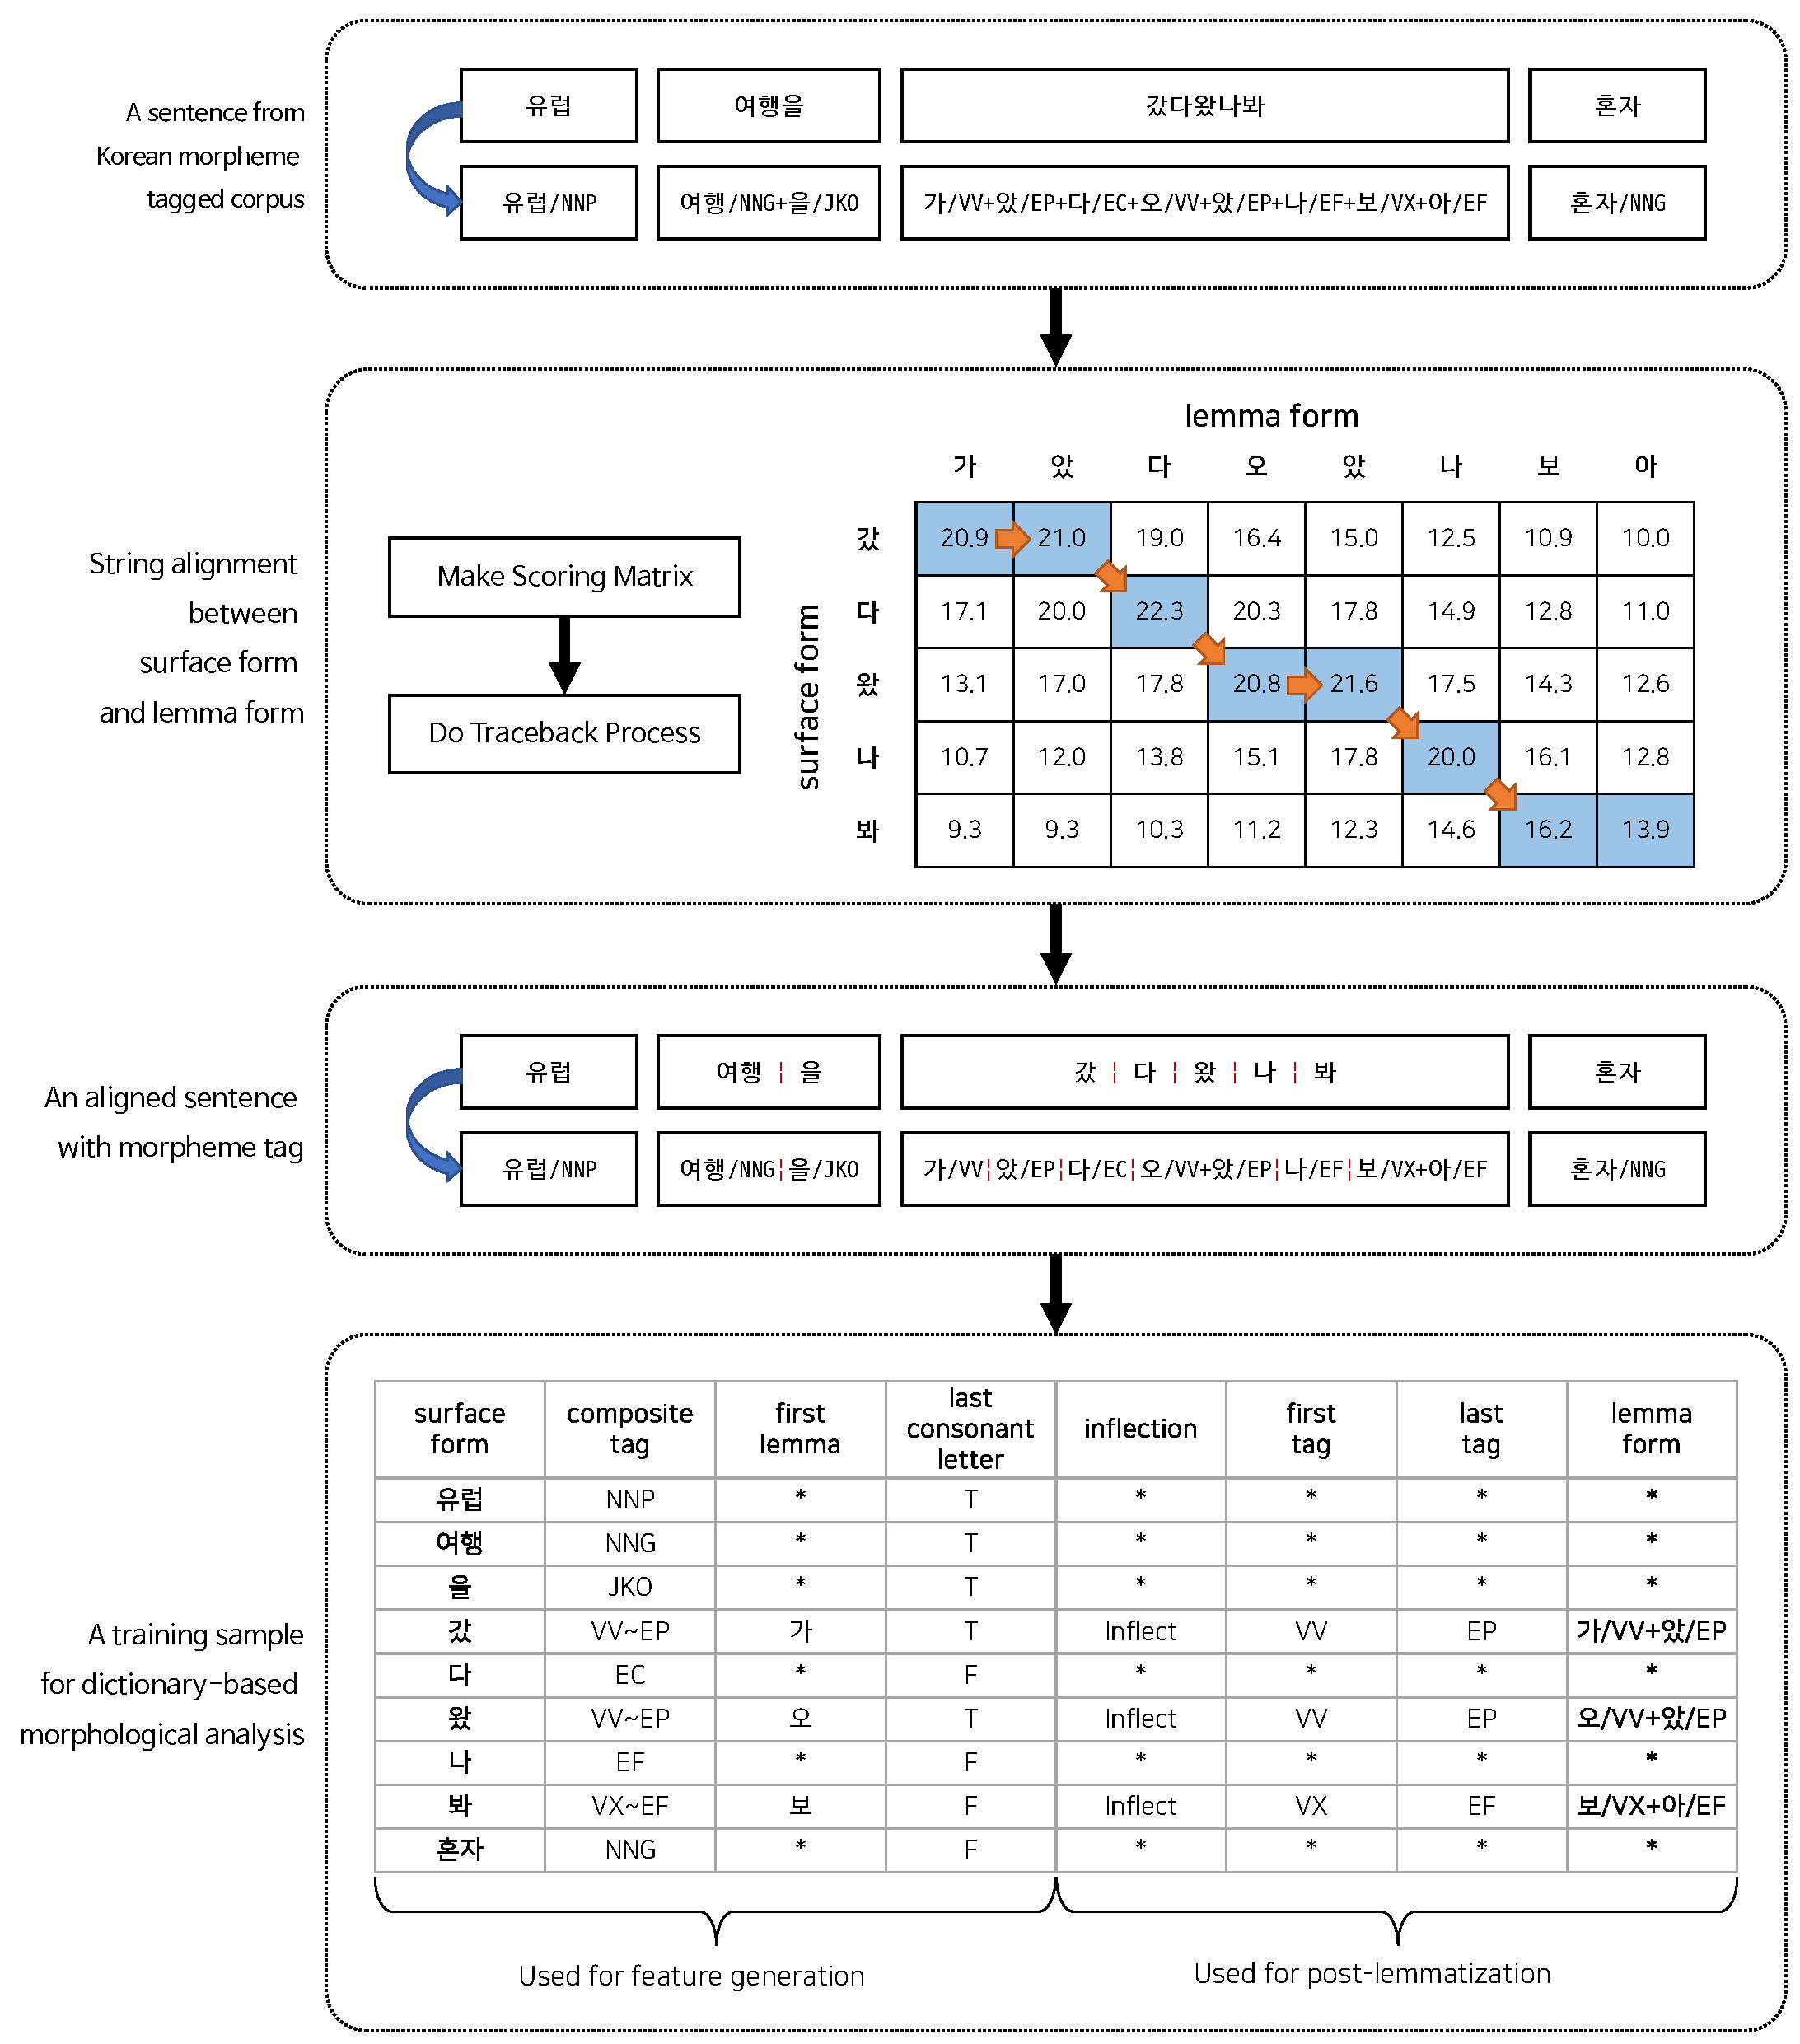
\includegraphics[width=0.5\textwidth]{img/fig1}}
        \caption{The transformation of a single sentence in the Korean morphology tagged corpus into a single training sample}\label{fig:sample}
    \end{figure}

    In order to train a dictionary-based morpheme analysis model, it is necessary to make the morpheme tagged corpus, which is previously expressed in lemma form, into a form that includes boundary information between morphemes in surface form.
    In this process, a string alignment method that considers the difference between the lemma form and the surface form in the Korean morphological analysis corpus is essential.
    In this study, string alignment was performed with the Smith-Waterman algorithm using a scoring matrix based on the similarity in the grapheme unit of Korean letters for each word pair.
    (See Figure~\ref{fig:sample})
    One aligned sentence with morpheme tag can be transformed into one training sample for dictionary-based morphological analysis.
    In the tabular data at the bottom of Figure~\ref{fig:sample}, each line becomes a unit constituting a lexicon, the first four columns are used for feature generation and the last four columns used for post-lemmatization.

    %사전 기반 형태소 분석 모델을 학습하기 위해서는 기존에 lemma form으로 표현되어 있는 morpheme tagged corpus를 surface form에서의 형태소 간의 경계 정보가 포함된 형태로 만들어 줄 필요가 있다.
    %이 과정 내에서 한국어 형태 분석 말뭉치 내의 lemma form과 surface form 간의 차이를 고려한 string alignment 방법이 핵심적으로 필요하게 된다.
    %본 연구에서는 각 어절 쌍에 대해서 한국어 글자의 자소 단위에서의 유사도에 기반한 scoring matrix를 사용한 Smith-Waterman 알고리즘으로 문자열 정렬을 수행하였다.
    %(Figure~\ref{fig:sample} 참조)
    %하나의 aligned sentence with morpheme tag는 하나의 training sample for dictionary-based morphological analysis로 변형될 수 있게 된다.
    %Figure~\ref{fig:sample}의 하단에 있는 표 형태의 데이터에서 각 줄은 lexicon을 구성하는 단위가 되며, 전반의 4개 열은 feature generation에 사용되고 후반의 4개 열은 post-lemmatization에 사용된다.


    \section{Transformer-based Re-ranking Model}\label{sec4}

    Korean morphological analysis is the process of determining parts of speech by finding morphemes, which are the smallest units of language expression that have an independent meaning in a sentence.
    In an isolating language like English, this can be done relatively simply by tagging parts of speech sequentially, but in Korean, the nature of the agglutinative language requires separating endings or investigatives and restoring inflections to their original form.
    In addition, since the basic input of other Korean analysis tasks is often a separated morpheme, the accuracy of morphological analysis greatly affects the performance of Korean analysis.

    %학습된 형태소 분석 모델의 차선 결과들을 생성하여 재순위화 데이터를 만드는 방법


    \section{Experimental Results}\label{sec5}

    Korean morphological analysis is the process of determining parts of speech by finding morphemes, which are the smallest units of language expression that have an independent meaning in a sentence.
    In an isolating language like English, this can be done relatively simply by tagging parts of speech sequentially, but in Korean, the nature of the agglutinative language requires separating endings or investigatives and restoring inflections to their original form.
    In addition, since the basic input of other Korean analysis tasks is often a separated morpheme, the accuracy of morphological analysis greatly affects the performance of Korean analysis.

    %형태소 분석 모델 및 재순위화 모델을 통한 성능 개선 실험 결과


    \section{Error Analysis and Case Studies}\label{sec6}

    Korean morphological analysis is the process of determining parts of speech by finding morphemes, which are the smallest units of language expression that have an independent meaning in a sentence.
    In an isolating language like English, this can be done relatively simply by tagging parts of speech sequentially, but in Korean, the nature of the agglutinative language requires separating endings or investigatives and restoring inflections to their original form.
    In addition, since the basic input of other Korean analysis tasks is often a separated morpheme, the accuracy of morphological analysis greatly affects the performance of Korean analysis.

    %오류 분석 및 성능 개선 사례들


    \section{Conclusion}\label{sec7}

    Korean morphological analysis is the process of determining parts of speech by finding morphemes, which are the smallest units of language expression that have an independent meaning in a sentence.
    In an isolating language like English, this can be done relatively simply by tagging parts of speech sequentially, but in Korean, the nature of the agglutinative language requires separating endings or investigatives and restoring inflections to their original form.
    In addition, since the basic input of other Korean analysis tasks is often a separated morpheme, the accuracy of morphological analysis greatly affects the performance of Korean analysis.


    %결론과 향후 연구

    %\nocite{*}% Show all bib entries - both cited and uncited; comment this line to view only cited bib entries;
    \bibliography{WileyNJD-AMS}

    \section*{Author Biography}

    \begin{biography}{
\includegraphics[width=60pt,height=70pt,draft]{empty}}{\textbf{Author Name.} This is sample author biography text this is sample author biography text this is sample author biography text this is sample author biography text this is sample author biography text this is sample author biography text this is sample author biography text this is sample author biography text this is sample author biography text this is sample author biography text this is sample author biography text this is sample author biography text this is sample author biography text this is sample author biography text this is sample author biography text this is sample author biography text this is sample author biography text this is sample author biography text this is sample author biography text this is sample author biography text this is sample author biography text.}
    \end{biography}

\end{document}
